\documentclass[a4paper, 10pt]{article}

\usepackage{graphicx}
\graphicspath{{public/}}

\usepackage{geometry}
\geometry{left=1.5cm, right=1.5cm, top=3cm, bottom=2cm}

\usepackage{array}
\usepackage{listings}
\usepackage{color}


\newcommand{\tabincell}[2]{\begin{tabular}{@{}#1@{}}#2\end{tabular}}

\lstset{
    backgroundcolor=\color[RGB]{245,245,244}    
}

\begin{document}
\title{\textbf{MapReduce Assignment}}
\author{\textit{Submitted By: Ujjawal Sharma}}
\date{}
\maketitle

\section{Overview}
\noindent
MapReduce is a software framework which can help us to write applications which can process a large amount of data in parallel on large clusters in a reliable and fault tolerant manner.

MapReduce job splits the main task into two different tasks namely mapper and reducer. A mapper task processes the input data provided by the user independent of that of reducer task and post the processing, it passes its output to the reducer task. The reducer task then processes the input received from the mapper task and provide us with its own output. Both the input and output is stored in a file system. The framework takes care of scheduling tasks, monitoring them and re-executes the failed tasks.

Mostly, the compute nodes and the storage nodes are the same, that is, the MapReduce framework and the Hadoop Distributed File System are running on the same set of nodes.

For using the MapReduce framework, I used the Hadoop Streaming Utility which comes with the Hadoop distribution. The Streaming API helps to execute any code or script which are created for the purpose of mapping or reducing. The streamming utility creates a Map/Reduce job, submits the job to any particular cluster and then monitor the progress of the job. 

\section{Hadoop Setup}

For understanding the MapReduce Framework using the Hadoop's streaming API, I followed the steps provided at the below link:

\begin{lstlisting} [
    basicstyle=\small, %or \small or \footnotesize etc.
]
http://hadoop.apache.org/docs/stable/hadoop-project-dist/hadoop-common/SingleCluster.html
\end{lstlisting}

For the basic understanding of the working of MapReduce, i installed the Standalone mode of Hadoop which is used for standalone operations.

After following the steps provide in the above link, i was able to access the below URL through my Web-Browser, which confirmed the successful installation of hadoop on my system:
\begin{lstlisting} [
    basicstyle=\small, %or \small or \footnotesize etc.
]
http://localhost:50070/
\end{lstlisting}

\begin{figure}[!htbp]
    \centering
    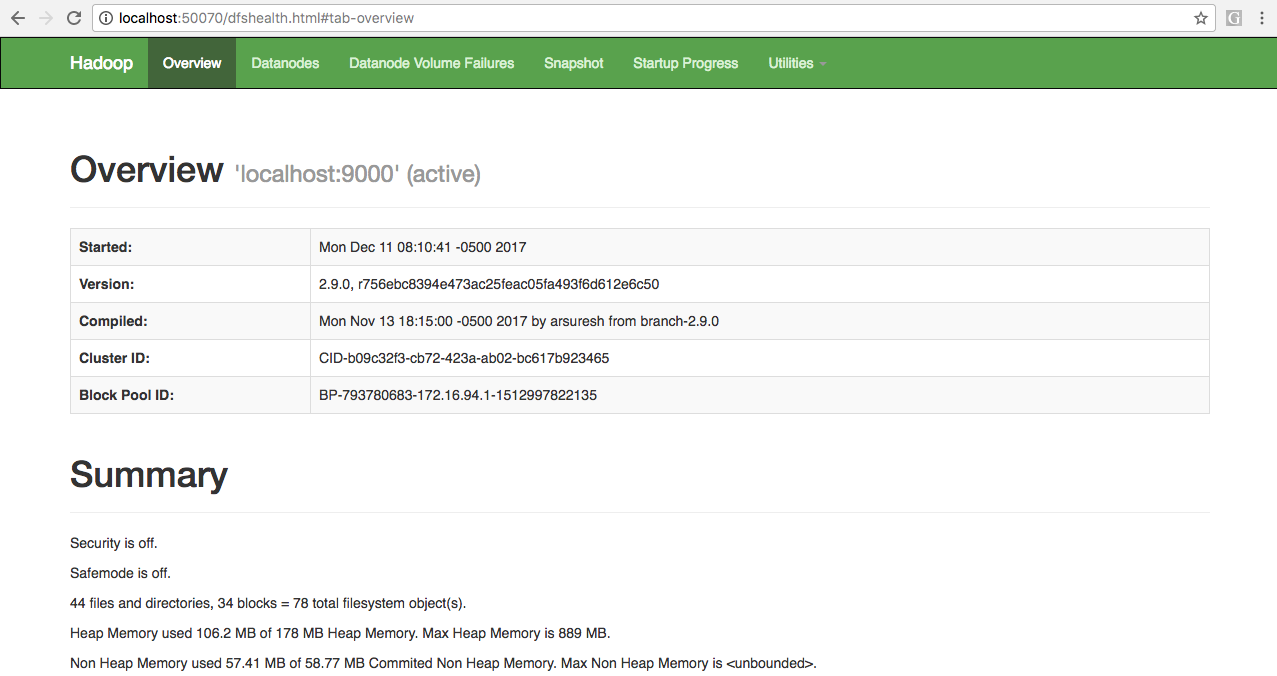
\includegraphics[height=7cm]{InstallationConfirmation.png}
    \caption{Hadoop Installation Confirmation}
\end{figure}
\newpage

Post the installation I created the HDFS directories which are responsible for running the MapReduce jobs following the steps provided in the same link of installation(provided above).

\section{Questions and Solutions}
\subsection{Question 1}
\textbf{On how many occasions did companies violate the DoNotCallRegistry?}\\
\noindent
\textbf{Solution:}
The mapper class below has a doNotCallNumbers list initiated which keeps the numbers which are registered for Do Not Call. Our mapper class will takes the call-log file as the input, reading it line by line and verifies if the recipient of any call is one of those numbers available in the doNotCallNumbers list. If the number is present, it will output the Company's name which is violating the DoNotCallRegistry.
The output is then passed to the Reducer class.

\begin{lstlisting}[language=Python, caption=Mapper for problem 1]
    #!/usr/bin/env python
    import sys
    
    doNotCallNumbers = ["2166849356","4049345110","5893715037","9457920329"]

    #Iterating over each line
    for line in sys.stdin:
        line = line.strip()

        #Splitting each line on the basis of delimiter.
        words = line.split(";")

        #Printing the output
        if words[3].strip() in doNotCallNumbers:
            print '%s\t\t%s' % (words[1],1)       
\end{lstlisting}

The reducer class reads the output provided by mapper class line by line and stores the count of number of violations made by each company in a dictionary. Finally, the items in the dictionary are sorted so as to output the names of companies in an alphabetical order. The output will also contains the number of times each company violated the DoNotCallRegistry.

\begin{lstlisting}[language=Python, caption=Reducer for problem 1]
    #!/usr/bin/env python
    import sys
    
    flagged_company_dict={}

    #Iterating over the inputs provided by mapper
    for line in sys.stdin:
        line = line.strip()

        #Splitting the input based on delimiter
        companyName, count = line.split('\t', 1)

        #Doing the count for each company occurance
        if companyName in flagged_company_dict:
                newCount=flagged_company_dict.get(companyName)+1
                flagged_company_dict.update({companyName:newCount}) 
        else:
                flagged_company_dict.update({companyName:1})

    #Sorting and printing the output        
    for key,value in sorted(flagged_company_dict.items()):
        print '%s\t%s' %(key,value)            
\end{lstlisting}

\noindent
\textbf{Running the python code through terminal:}
\begin{figure}[!htbp]
    \centering
    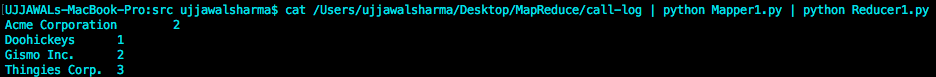
\includegraphics[height=1.5cm]{Question1.png}
    \caption{Output through terminal run}
\end{figure}

\noindent
\textbf{Running the python code through hadoop streaming API:}
\begin{figure}[!htbp]
    \centering
    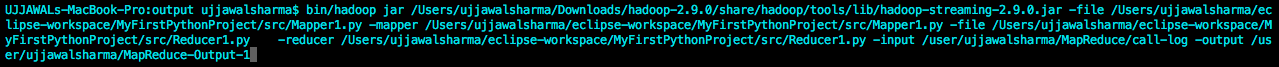
\includegraphics[height=1cm]{Run1.png}
    \caption{Running through streaming API}
\end{figure}

\noindent
\textbf{Output on Hadoop HDFS:}
\begin{figure}[!htbp]
    \centering
    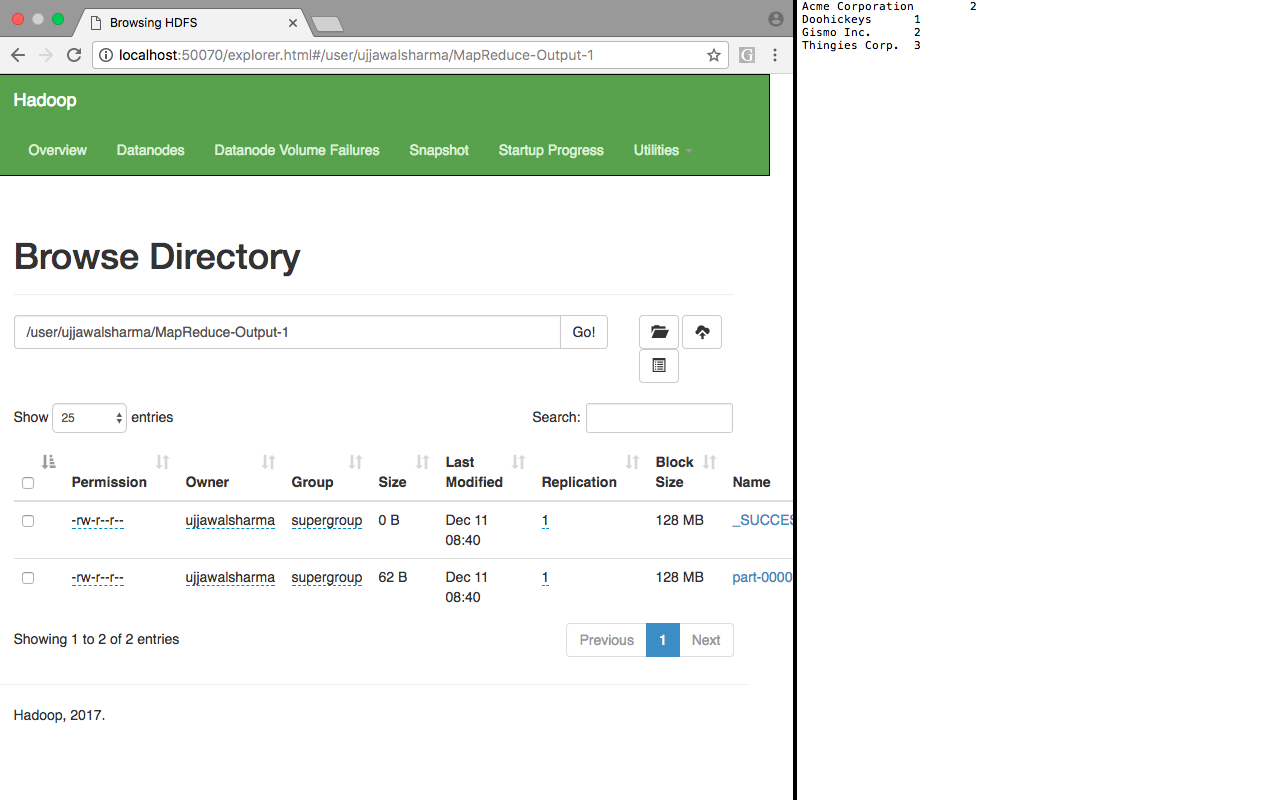
\includegraphics[height=10cm]{Hadoop1.png}
\end{figure}

\subsection{Question 2}
\textbf{How many numbers should be blocked/marked as spam to reduce the number of unwanted calls?}\\
\noindent
\textbf{Solution:}
The mapper class here is using the same doNotCallNumbers list to store the list of numbers which are registered for doNotCall. Another dictionary is created which keep the count of how many calls were placed by each company. The STDIN iterator reads through each line of the call-log file and keeps the occurances of each company in the companyCount dictionary. After the dictionary is populated with the values, the iterator also verifies the recipient of each call statement and if the numbers are one of those present in the doNotCallNumbers list, the name of the company is stored in the flaggedCompany list. Finally, the output is provided by printing the flaggedCompany list and companyCount dictionary.

\begin{lstlisting}[language=Python, caption=Mapper for problem 2]
    #!/usr/bin/env python
    import sys
    
    flaggedCompany=[]
    doNotCallNumbers = ["2166849356","4049345110","5893715037","9457920329"]
    companyCount={}

    #Iterating over each line
    for line in sys.stdin:
        line = line.strip()

        #Splitting each line on the basis of delimiter
        words = line.split(";")

        #Adding the count of each company to dictionary
        if words[1] in companyCount:
            newCount=companyCount.get(words[1])+1
            companyCount.update({words[1]:newCount}) 
        else:
            companyCount.update({words[1]:1})

        #Storing the flagged companies   
        if (words[3].strip() in doNotCallNumbers):
            flaggedCompany.append(words[1])
    
    #Printing the output      
    flaggedCompany=list(set(flaggedCompany))
    print '%s\t%s' %(flaggedCompany,companyCount)  
\end{lstlisting}

The reducer class reads the output provided by mapper class (the flaggedCompany list and companyCount dictionary), and do some string manipulation (please see the code block). Finally, it prints the output as shown in below images.

\begin{lstlisting}[language=Python, caption=Reducer for problem 2]
    #!/usr/bin/env python
    import sys
    companyList=[]
    companyDict=[]

    #Iterating over the inputs provided by mapper
    for line in sys.stdin:
        line = line.strip()

        #Splitting the input based on delimiter
        companyNameList, finalCountDict = line.split('\t', 1)

        #String Manipulation
        companyNameList=companyNameList.replace("[","")
        companyNameList=companyNameList.replace("]","")
        companyNameList=companyNameList.replace(" '","")
        companyNameList=companyNameList.replace("'","")
        companyList=companyNameList.strip().split(",")
      
        finalCountDict=finalCountDict.replace("{","")
        finalCountDict=finalCountDict.replace("}","")
        finalCountDict=finalCountDict.replace("'","")
        finalCountDict=finalCountDict.replace(", ",",")
        finalCountDict=finalCountDict.replace(": ",":")
        companyDict=finalCountDict.split(",");
        companyList.sort()
        
        #Iterating over each item and printing the output
        for listItem in companyList:
            for dictItem in companyDict:
                if listItem in dictItem:
                    print dictItem.replace(":","\t")           
\end{lstlisting}

\noindent
\textbf{Running the python code through terminal:}
\begin{figure}[!htbp]
    \centering
    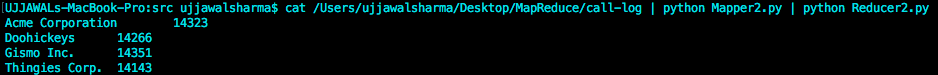
\includegraphics[height=1.5cm]{Question2.png}
    \caption{Output through terminal run}
\end{figure}

\noindent
\textbf{Running the python code through hadoop streaming API:}
\begin{figure}[!htbp]
    \centering
    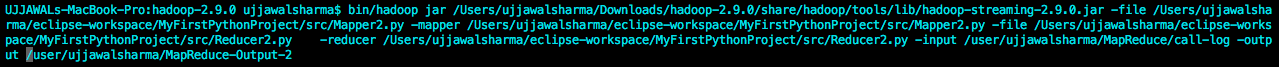
\includegraphics[height=1cm]{Run2.png}
    \caption{Running through streaming API}
\end{figure}

\noindent
\textbf{Output on Hadoop HDFS:}
\begin{figure}[!htbp]
    \centering
    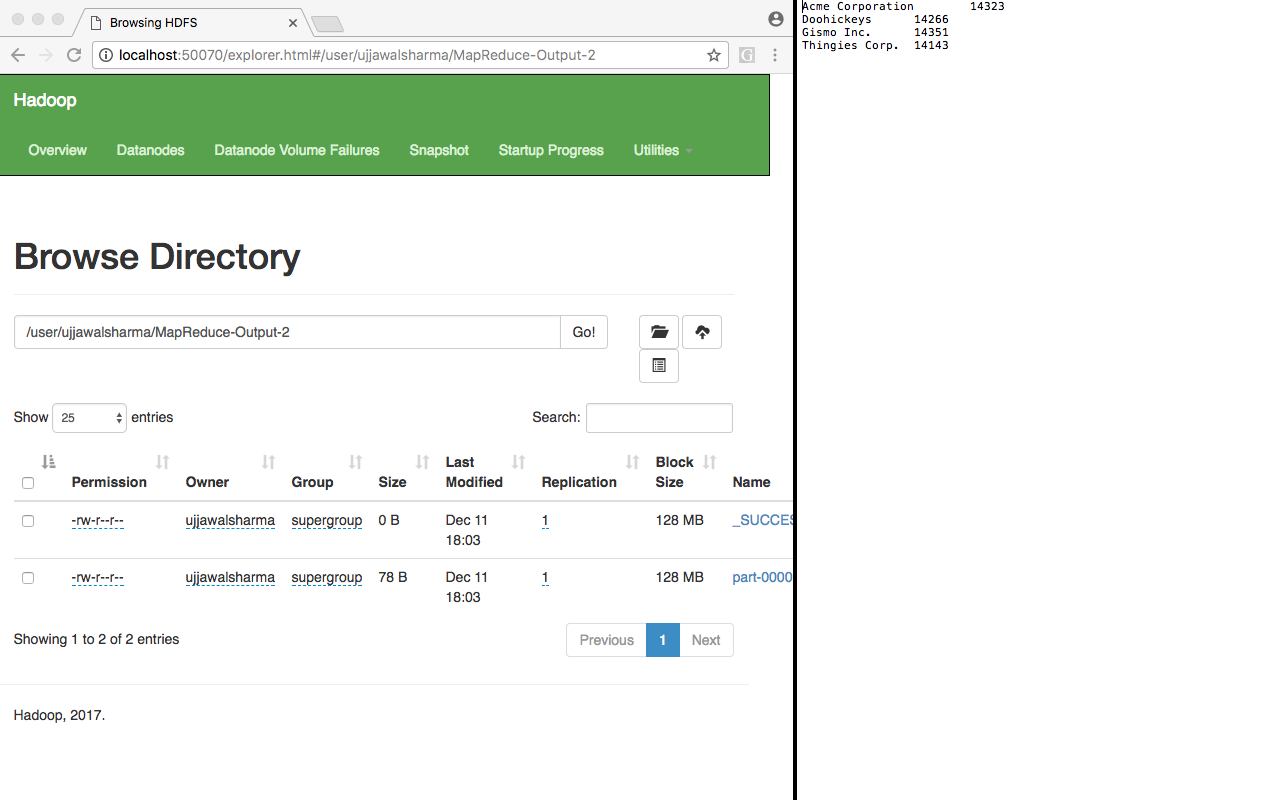
\includegraphics[height=10cm]{Hadoop2.png}
\end{figure}

\subsection{Question 3}
\textbf{Which telephone numbers received the most spam calls?}\\
\noindent
\textbf{Solution:}
The mapper class for this problem takes the input from the call-log file, one-by-one and verifies if the recipient of the call statement is present in the doNotCallNumbers list. If the number is available in the list, then the iterator puts the corresponding company name in the flaggedCompany list. Also, the iterator keeps on adding each call statement to a list called listofline.\\
\newpage
This list is later used to mark the call statement as Flagged, if the company's name of the statement is present in the flaggedCompany list. The final output is a list of recipient, each followed by a tab of space and the keyword Flagged. This output is passed to the Reducer class.

\begin{lstlisting}[language=Python, caption=Mapper for problem 3]
    #!/usr/bin/env python
    import sys
    
    flaggedCompany=[]
    doNotCallNumbers = ["2166849356","4049345110","5893715037","9457920329"]
    list_of_line=[]

    #Iterating over input lines
    for line in sys.stdin:
        list_of_line.append(line)
        line = line.strip()

        #Splitting each line on the basis of delimiter
        words = line.split(";")

        #Preparing the flagged company list
        if (words[3].strip() in doNotCallNumbers):
            flaggedCompany.append(words[1]) 
        
    flaggedCompany=list(set(flaggedCompany))   
    
    #If company is a flaggedcompany, print the output
    for item in list_of_line:
        list_line = item.strip()
        list_words = item.split(";")
        if list_words[1] in flaggedCompany:
            print '%s\t%s' %(list_words[3],"Flagged")         
\end{lstlisting}

The reducer class reads the output provided by mapper class (something like:"5795054160 Flagged") and then keeps the count of occurances of each recipient in the recipientDictionary. Finally, the list of top 3 recipients is printed.

\begin{lstlisting}[language=Python, caption=Reducer for problem 3]
    #!/usr/bin/env python
    import sys
    companyList=[]
    recipient_list=[]
    recipientDictionary={}
    maximumRecipient=[]

    #Iterating over the inputs provided by mapper
    for line in sys.stdin:
        line = line.strip()

        #Splitting the input based on delimiter
        obtainedValues = line.split('\t')
        recipient=""
        flag=""
        recipient_list.append(obtainedValues[0])

    #Iterating over each input to update recipient count in dictionary
    for item in recipient_list:
        recipient=item
        if recipient in recipientDictionary:
                newCount=recipientDictionary.get(recipient)+1
                recipientDictionary.update({recipient:newCount}) 
        else:
                recipientDictionary.update({recipient:1})
        
    for item in recipientDictionary:
        maximumRecipient.append(recipientDictionary.get(item))

    #Populating the maximum count table with top 3 values
    maximumRecipient=list(set(maximumRecipient))
    newList=sorted(maximumRecipient, reverse=True)[:3]
    
    #Printing the output for the top-3 values
    for count in newList:
        for item in recipientDictionary:
            if recipientDictionary.get(item)==count:
                mobile_number=item
                mobile_number=mobile_number[:6] + '-' + mobile_number[6:]
                mobile_number=mobile_number[:3] + ' ' + mobile_number[3:]
                mobile_number=mobile_number[:0] + '(' + mobile_number[0:]
                mobile_number=mobile_number[:4] + ')' + mobile_number[4:]
                print '%s\t%s' %(mobile_number,count)
         
\end{lstlisting}

\noindent
\textbf{Running the python code through terminal:}
\begin{figure}[!htbp]
    \centering
    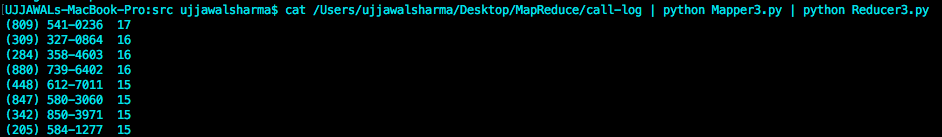
\includegraphics[height=2.5cm]{Question3.png}
    \caption{Output through terminal run}
\end{figure}

\noindent
\textbf{Running the python code through hadoop streaming API:}
\begin{figure}[!htbp]
    \centering
    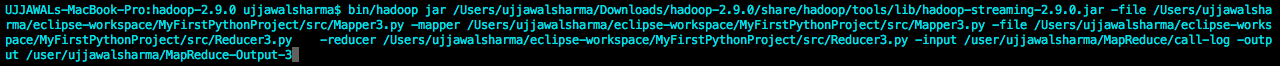
\includegraphics[height=1cm]{Run3.png}
    \caption{Running through streaming API}
\end{figure}

\newpage
\noindent
\textbf{Output on Hadoop HDFS:}
\begin{figure}[!htbp]
    \centering
    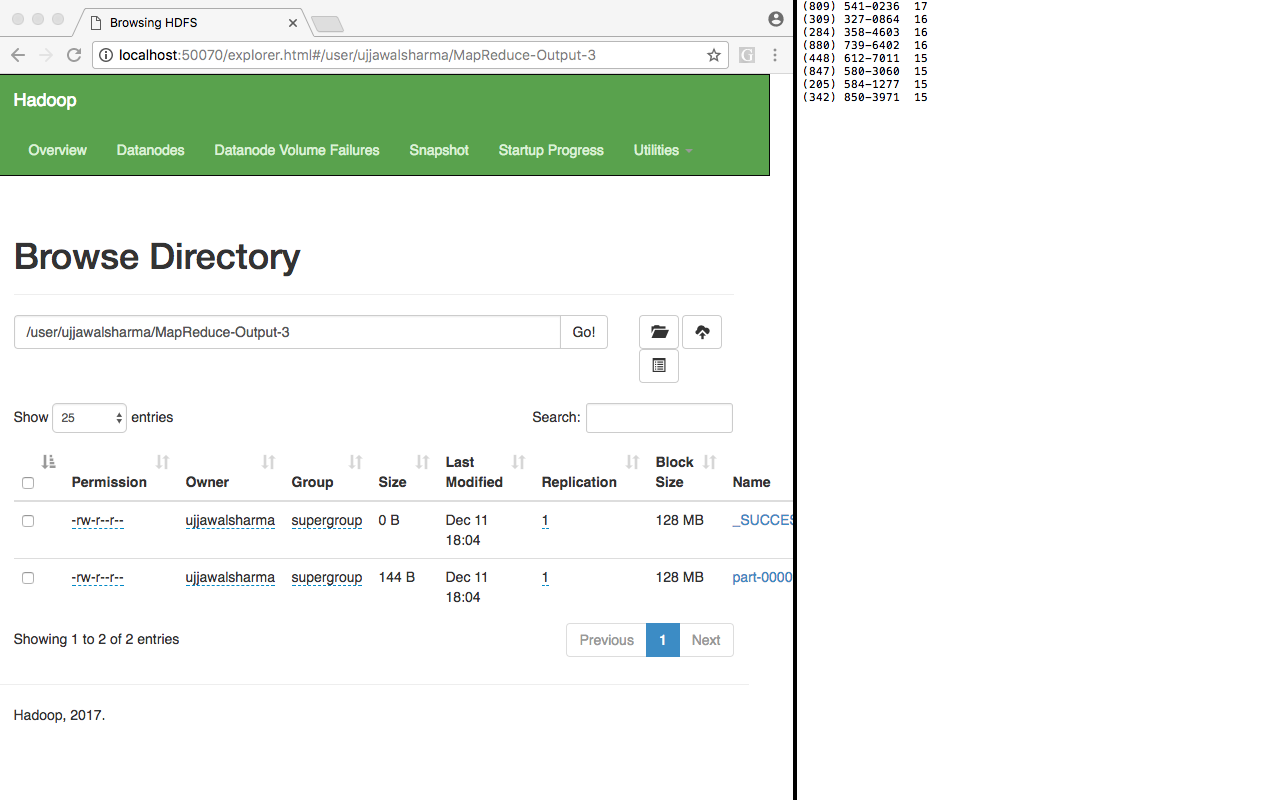
\includegraphics[height=10cm]{Hadoop3.png}
\end{figure}

\subsection{Question 4}
\textbf{Which telephone numbers are responsible for the most spam calls?}\\
\noindent
\textbf{Solution:}
The STDIN input iterator of mapper class takes the input from the call-log line one-by-one and stores each line in a list named linelist. It also verifies if recipient of any call statement is a member of doNotCallNumbers. If the number is a member of the doNotCallNumbers list, the iterator stores the corresponding companies name in flaggedCompanies list.

Another iterator is run for the linelist list which verifies if the company name corresponding to each call is a member of flaggedCompanies. if it is a member of flaggedCompanies, the iterator outputs the caller number and 1 as the output which is passed to the reducer class. 


\begin{lstlisting}[language=Python, caption=Mapper for problem 4]
    #!/usr/bin/env python
    import sys
    
    doNotCallNumbers = ["2166849356","4049345110","5893715037","9457920329"]
    flaggedCompanies=[]
    line_list=[]
    
    #Iterating over the inputs
    for line in sys.stdin:
        line_list.append(line)
        line = line.strip()

        #Splitting each word on the basis of delimiter
        words = line.split(";")

        #Preparing list of flagged companies
        if words[3].strip() in doNotCallNumbers:
            flaggedCompanies.append(words[1])
    
    #If Company name is flagged, print the caller
    for line_from_list in line_list:
        line_from_list = line_from_list.strip()
        words_of_line_from_list = line_from_list.split(";")
        if words_of_line_from_list[1] in flaggedCompanies:
            print '%s\t%s' %(words_of_line_from_list[2],1)        
\end{lstlisting}

The reducer class reads each line as the input provided by the mapper and stores the caller numbers of each line to callerlist list.
Another iterator iterates over callerlist and stores the occurances of each caller as count in the callerDictionary. Finally, the top 3 callers list is produced as output.

\begin{lstlisting}[language=Python, caption=Reducer for problem 4]
    #!/usr/bin/env python
    import sys
    companyList=[]
    caller_list=[]
    callerDictionary={}
    maximumRecipient=[]

    #Iterating over the inputs provided by mapper
    for line in sys.stdin:
        line = line.strip()

        #Splitting the input based on delimiter
        obtainedValues = line.split('\t')
        caller=""
        flag=""
        caller_list.append(obtainedValues[0])
    
    #Storing the calling count of each number in dictionary  
    for item in caller_list:
        caller=item
        if caller in callerDictionary:
            newCount=callerDictionary.get(caller)+1
            callerDictionary.update({caller:newCount}) 
        else:
            callerDictionary.update({caller:1})
            
    for item in callerDictionary:
        maximumRecipient.append(callerDictionary.get(item))

    #Populating the maximum list and sorting
    maximumCaller=list(set(maximumRecipient))
    newList=sorted(maximumCaller, reverse=True)[:3]
    
    #Printing the output for top 2 values
    for count in newList:
        for item in callerDictionary:
            if callerDictionary.get(item)==count:
                mobile_number=item
                mobile_number=mobile_number[:6] + '-' + mobile_number[6:]
                mobile_number=mobile_number[:3] + ' ' + mobile_number[3:]
                mobile_number=mobile_number[:0] + '(' + mobile_number[0:]
                mobile_number=mobile_number[:4] + ')' + mobile_number[4:]
                print '%s\t%s' %(mobile_number,count)
                       
\end{lstlisting}

\newpage
\noindent
\textbf{Running the python code through terminal:}
\begin{figure}[!htbp]
    \centering
    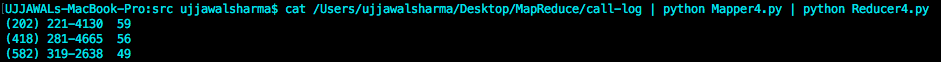
\includegraphics[height=1.2cm]{Question4.png}
    \caption{Output through terminal run}
\end{figure}

\noindent
\textbf{Running the python code through hadoop streaming API:}
\begin{figure}[!htbp]
    \centering
    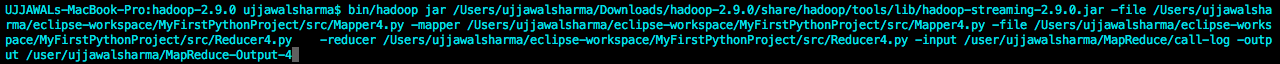
\includegraphics[height=1cm]{Run4.png}
    \caption{Running through streaming API}
\end{figure} 


\noindent
\textbf{Output on Hadoop HDFS:}
\begin{figure}[!htbp]
    \centering
    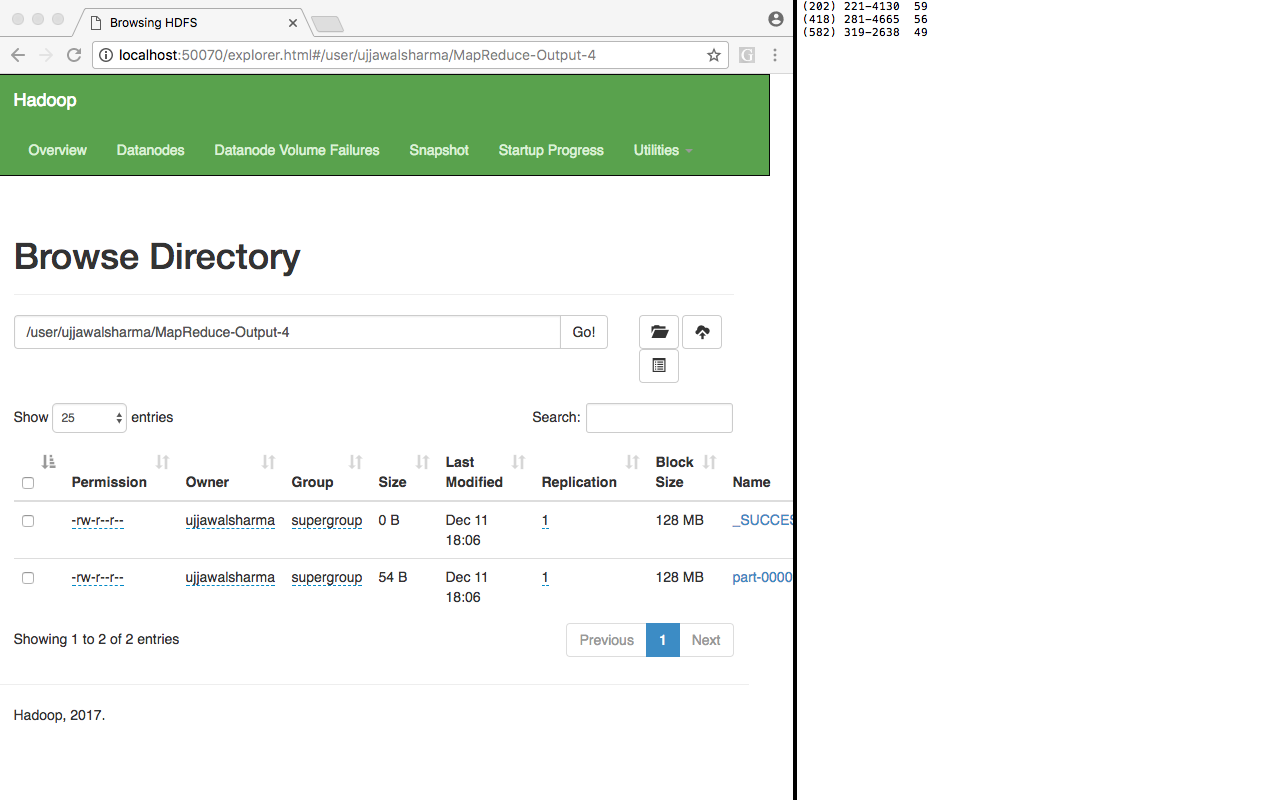
\includegraphics[height=10cm]{Hadoop4.png}
\end{figure}

\subsection{Question 5}
\textbf{Which telephone numbers received the most spam calls?}\\
\noindent
\textbf{Solution:}
The mapper firstly iterates over each line of input from STDIN and stores it in linelist list and also populates the flaggedCompanies list.
Finally the timestamp value of each call record is printed as output to the reducer with 1(serving as the count). 

\begin{lstlisting}[language=Python, caption=Mapper for problem 5]
    #!/usr/bin/env python
    import sys
    
    doNotCallNumbers = ["2166849356","4049345110","5893715037","9457920329"]
    flaggedCompanies=[]
    line_list=[]

    #Iterating over each input line
    for line in sys.stdin:
        line_list.append(line)
        line = line.strip()

        #Splitting each line on the basis of delimiter.
        words = line.split(";")

        #Preparing the flagged company list
        if words[3].strip() in doNotCallNumbers:
            flaggedCompanies.append(words[1])
    
    flaggedCompanies=list(set(flaggedCompanies))
    
    #printing the timestamp as the output
    for line_in_line_list in line_list:
        line_in_line_list = line_in_line_list.strip()
        words_in_line_list = line_in_line_list.split(";")
        print '%s\t%s' %(words_in_line_list[0],1)   
\end{lstlisting}

The reducer takes the input provided by mapper and stores the hour value of each record in the hourlist list.
Another iterator iterates over this list and stores the occurances of each hour value in the hourdictionary.
Finally, the top-3 time period getting the maximum calls is produced as output.

\begin{lstlisting}[language=Python, caption=Reducer for problem 5]
    #!/usr/bin/env python
    import sys
    
    hour_dictionary={}
    hour_list=[]
    count_list=[]

    #Iterating over the inputs provided by mapper
    for line in sys.stdin:
        line = line.strip()

        #Splitting the input based on delimiter
        obtainedTimeString = line.split('\t')
        caller=""
        flag=""
        onlyTime=obtainedTimeString[0].split(" ")
        hour_value=onlyTime[1].split(":")
        hour_list.append(hour_value[0])
    
    #Storing the count of each hour in the dictionary   
    for item in  hour_list:
        if item in hour_dictionary:
            newCount=hour_dictionary.get(item)+1
            hour_dictionary.update({item:newCount}) 
        else:
            hour_dictionary.update({item:1}) 
    
    for item in hour_dictionary:
        count_list.append(hour_dictionary.get(item))
    
    maximum_list=sorted(count_list, reverse=True)[:3]
    
    #getting the maximum 3 top values
    reverse_sorted_list=[]
    while maximum_list:
        maximum = maximum_list[0]  # arbitrary number in list 
        for x in maximum_list: 
            if x > maximum:
                maximum = x
        reverse_sorted_list.append(maximum)
        maximum_list.remove(maximum) 
    
    #Printing the top 3 values in the required way
    for reverse_item in reverse_sorted_list:
        for item in hour_dictionary:
            if hour_dictionary.get(item) == reverse_item:
                time=int(item)
                suffix=""
                if time<12:
                    suffix=" am"
                if time==12:
                    suffix=" noon"
                if time>12:
                    time=time-12
                    suffix=" pm"
                time_value=str(time)+suffix   
                print '%s\t%s' %(time_value,hour_dictionary.get(item))
                            
\end{lstlisting}
\noindent
\textbf{Running the python code through terminal:}
\begin{figure}[!htbp]
    \centering
    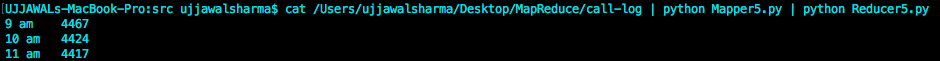
\includegraphics[height=1.2cm]{Question5.png}
    \caption{Output through terminal run}
\end{figure}

\noindent
\textbf{Running the python code through hadoop streaming API:}
\begin{figure}[!htbp]
    \centering
    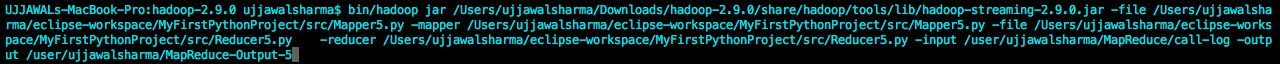
\includegraphics[height=0.90cm]{Run5.png}
    \caption{Running through streaming API}
\end{figure}

\newpage
\noindent
\textbf{Output on Hadoop HDFS:}
\begin{figure}[!htbp]
    \centering
    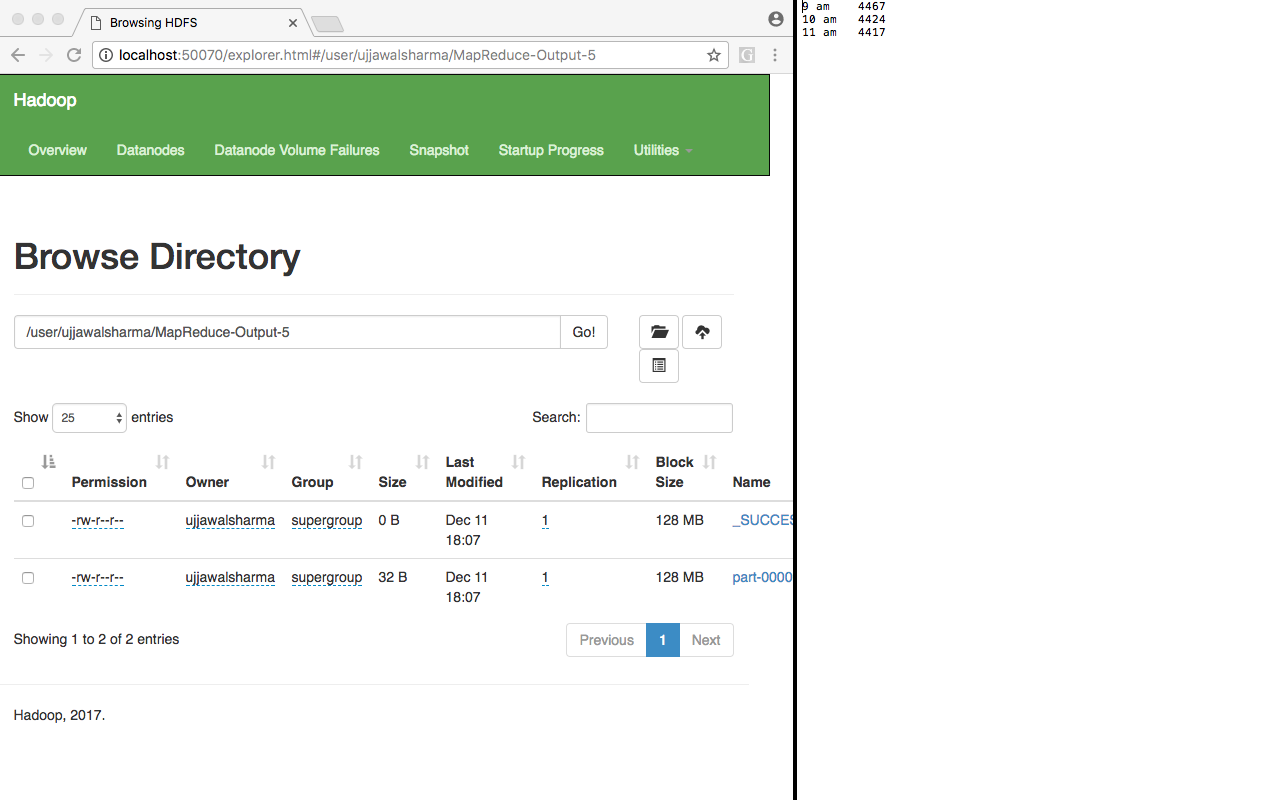
\includegraphics[height=10cm]{Hadoop5.png}
\end{figure}

\section{Conclusion}

All the programs ran successfully through both python and hadoop streaming API and I was able to get same results on both the platform. According to the description of Hadoop streaming API, I was able to get the output of each problem in a file format as well.

\end{document}